% You can copy this file for every new figure.
%
% Figures should be placed at the top of pages/columns
% where they can.
%
% This can be ensured by using the [t] parameter to the
% "\begin{figure}" declaration.
%
\begin{figure}[t]
    % Figures should be centered in the page/column
    \centering
    %
    % Figure content goes here. This could be a graphic,
    % a TikZ diagram, etc.
    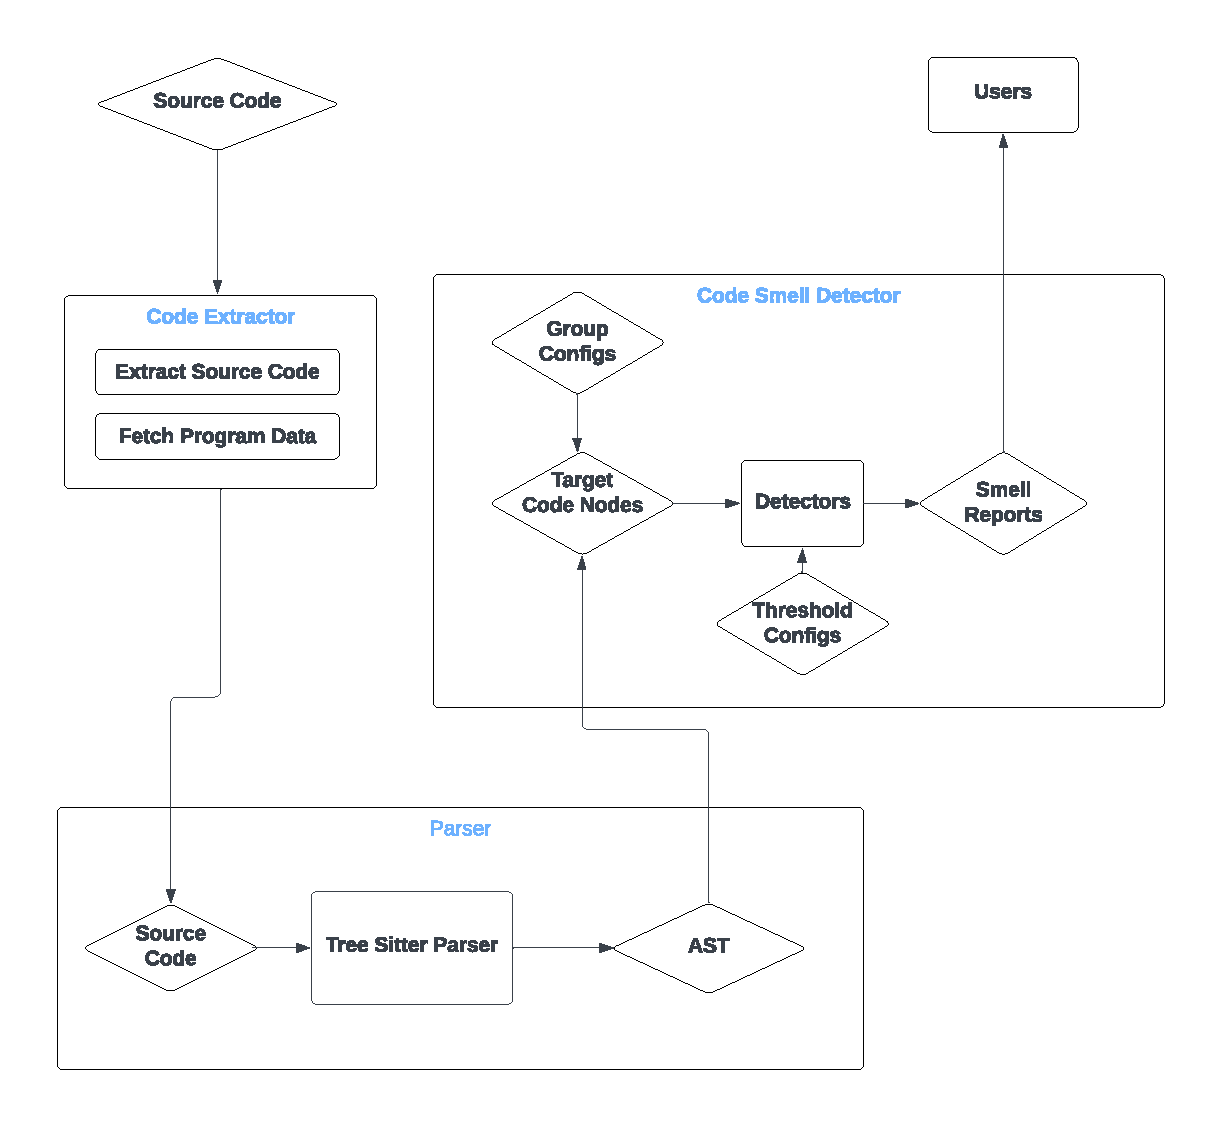
\includegraphics[width=\columnwidth]{graphics/Architecture.pdf}
    %
    % Depending on the template, some breathing space might need to
    % be added (use \smallskip \medskip etc.) here
    %
    % Or, to save space, you might want to remove space
    % (use a negative \vspace, e.g. \vspace{-1em})
    %
    \caption{
        % The label should appear _inside_ the caption to ensure
        % Latex numbers it correctly. This is a common gotcha!
        %
        % All figure labels should start with "fig:"
        % So that the figure file can be found easily, the rest of the
        % figure label should be the same as the filename, as it is
        % in this example:
        %
        \label{fig:architecture}
        %
        TreeNose: the Code Smell Detection Architecture 
    }
    %
    % To save space, you might want to remove space here
    % (use a negative \vspace, e.g. \vspace{-1em})
\end{figure}